\documentclass[12pt]{article}

\usepackage{tikz}
\usepackage{slashbox}
\usepackage{caption}
\usetikzlibrary{automata, positioning}
\begin{document}
	\begin{enumerate}
	\item
	The state diagram is like below:
	
	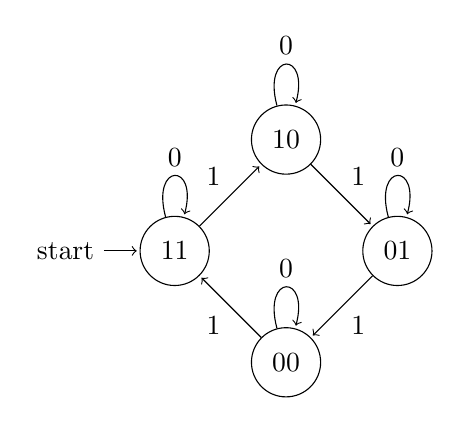
\begin{tikzpicture}[shorten >=1pt,node distance=2cm,on grid,auto] 
    	\node[state,initial] (11) {11}; 
    	\node[state] (10) [above right=of 11] {10}; 
    	\node[state] (00) [below right=of 11] {00}; 
    	\node[state](01)  [above right=of 00] {01};
    	\path [->]
    	(11) edge node {1} (10)
    	     edge [loop above] node {0} ()
    	(10) edge node {1} (01)
    	     edge [loop above] node {0} ()
    	(01) edge node {1} (00)
    	     edge [loop above] node {0} ()
    	(00) edge node {1} (11)
    	     edge [loop above] node {0} ();    	         
	\end{tikzpicture}	
	
	The state table is like the following:
	
	\begin{tabular}{c|cc}

		$x$ & Current State & Next State\\ \hline
		0 & 00 & 00\\ 
		0 & 01 & 01\\ 
		0 & 10 & 10\\ 
		0 & 11 & 11\\ 		
		1 & 00 & 11\\ 
		1 & 01 & 00\\ 
		1 & 10 & 01\\ 
		1 & 11 & 10\\ 
	\end{tabular}
	\begin{center}
	

	\begin{tabular}{|c|c|c|c|c|}
	\hline
	\backslashbox{x}{Current State} & 00 & 01 & 11 & 10 \\ \hline
	0 &0&0&1&1\\ \hline
	1 &1&0&1&0\\ \hline

	\end{tabular}		
	\end{center}
	\captionof{table}{Karnugh Map for $D_2$}		
	
	
	\begin{center}
	\begin{tabular}{|c|c|c|c|c|}
	\hline
	\backslashbox{x}{Current State} & 00 & 01 & 11 & 10 \\ \hline
	0 &0&1&1&0\\ \hline
	1 &1&0&0&1\\ \hline

	\end{tabular}		
	\end{center}
	\captionof{table}{Karnugh Map for $D_2$}
	
	\item
	\end{enumerate}
	
\end{document}